\documentclass{article}
%%%%%%%%%%%%%%%%%%%%%%%%%%%%% Define Article %%%%%%%%%%%%%%%%%%%%%%%%%%%%%%%%%%
%%%%%%%%%%%%%%%%%%%%%%%%%%%%%%%%%%%%%%%%%%%%%%%%%%%%%%%%%%%%%%%%%%%%%%%%%%%%%%%

%%%%%%%%%%%%%%%%%%%%%%%%%%%%% Using Packages %%%%%%%%%%%%%%%%%%%%%%%%%%%%%%%%%%
\usepackage{float}
\usepackage[letterpaper,portrait]{geometry}
\usepackage{graphicx}
\usepackage{anysize}
\usepackage{lipsum}
\usepackage{amsmath,amssymb,amsthm}
\usepackage[utf8]{inputenc}
\usepackage{multirow}
\usepackage{csquotes}
\usepackage[spanish]{babel}
\usepackage{apacite}
\usepackage{multicol}
\usepackage{parskip}
\usepackage{setspace}
\usepackage{empheq}
\usepackage{mdframed}
\usepackage{booktabs}
\usepackage{lipsum}
\usepackage{graphicx}
\usepackage{color}
\usepackage{psfrag}
\usepackage{pgfplots}
\usepackage{bm}
\usepackage{tocloft}
\usepackage{lscape}
\usepackage{adjustbox}
\setlength{\tabcolsep}{1.505625pt}
\renewcommand{\arraystretch}{1.2}
%%%%%%%%%%%%%%%%%%%%%%%%%%%%%%%%%%%%%%%%%%%%%%%%%%%%%%%%%%%%%%%%%%%%%%%%%%%%%%%

% Other Settings

%%%%%%%%%%%%%%%%%%%%%%%%%% Page Setting %%%%%%%%%%%%%%%%%%%%%%%%%%%%%%%%%%%%%%%
\geometry{letterpaper, margin=2.54cm}

%%%%%%%%%%%%%%%%%%%%%%%%%% Define some useful colors %%%%%%%%%%%%%%%%%%%%%%%%%%
\definecolor{ocre}{RGB}{243,102,25}
\definecolor{mygray}{RGB}{243,243,244}
\definecolor{deepGreen}{RGB}{26,111,0}
\definecolor{shallowGreen}{RGB}{235,255,255}
\definecolor{deepBlue}{RGB}{61,124,222}
\definecolor{shallowBlue}{RGB}{235,249,255}
%%%%%%%%%%%%%%%%%%%%%%%%%%%%%%%%%%%%%%%%%%%%%%%%%%%%%%%%%%%%%%%%%%%%%%%%%%%%%%%

%%%%%%%%%%%%%%%%%%%%%%%%%% Define an orangebox command %%%%%%%%%%%%%%%%%%%%%%%%
\newcommand\orangebox[1]{\fcolorbox{ocre}{mygray}{\hspace{1em}#1\hspace{1em}}}
%%%%%%%%%%%%%%%%%%%%%%%%%%%%%%%%%%%%%%%%%%%%%%%%%%%%%%%%%%%%%%%%%%%%%%%%%%%%%%%

%%%%%%%%%%%%%%%%%%%%%%%%%%%% English Environments %%%%%%%%%%%%%%%%%%%%%%%%%%%%%
\newtheoremstyle{mytheoremstyle}{3pt}{3pt}{\normalfont}{0cm}{\rmfamily\bfseries}{}{1em}{{\color{black}\thmname{#1}~\thmnumber{#2}}\thmnote{\,--\,#3}}
\newtheoremstyle{myproblemstyle}{3pt}{3pt}{\normalfont}{0cm}{\rmfamily\bfseries}{}{1em}{{\color{black}\thmname{#1}~\thmnumber{#2}}\thmnote{\,--\,#3}}
\theoremstyle{mytheoremstyle}
\newmdtheoremenv[linewidth=1pt,backgroundcolor=shallowGreen,linecolor=deepGreen,leftmargin=0pt,innerleftmargin=20pt,innerrightmargin=20pt,]{theorem}{Theorem}[section]
\theoremstyle{mytheoremstyle}
\newmdtheoremenv[linewidth=1pt,backgroundcolor=shallowBlue,linecolor=deepBlue,leftmargin=0pt,innerleftmargin=20pt,innerrightmargin=20pt,]{definition}{Definition}[section]
\theoremstyle{myproblemstyle}
\newmdtheoremenv[linecolor=black,leftmargin=0pt,innerleftmargin=10pt,innerrightmargin=10pt,]{problem}{Problem}[section]
%%%%%%%%%%%%%%%%%%%%%%%%%%%%%%%%%%%%%%%%%%%%%%%%%%%%%%%%%%%%%%%%%%%%%%%%%%%%%%%

%%%%%%%%%%%%%%%%%%%%%%%%%%%%%%% Plotting Settings %%%%%%%%%%%%%%%%%%%%%%%%%%%%%
\usepgfplotslibrary{colorbrewer}
\pgfplotsset{width=8cm,compat=1.9}
%%%%%%%%%%%%%%%%%%%%%%%%%%%%%%%%%%%%%%%%%%%%%%%%%%%%%%%%%%%%%%%%%%%%%%%%%%%%%%%

%%%%%%%%%%%%%%%%%%%%%%%%%%%%%%% Title & Author %%%%%%%%%%%%%%%%%%%%%%%%%%%%%%%%
\author{Gustavo Vergara}
%%%%%%%%%%%%%%%%%%%%%%%%%%%%%%%%%%%%%%%%%%%%%%%%%%%%%%%%%%%%%%%%%%%%%%%%%%%%%%%

\begin{document}
\pgfplotsset{compat=1.18}
\setstretch{2}

\begin{titlepage}
	\centering
	\vspace{2.5cm}
	{\scshape \Large TALLER DE MÁQUINAS TÉRMICAS\par}
	\vspace{5cm}
	\textbf\large\scshape{\par}
	\vspace{0.5cm}
	{\Large Vergara Pareja Gustavo\par}
    {\Large Ramos Flórez Miguel\par}
	\vspace{5cm}
	{\scshape\Large Bernardo J. Luján E. \par}
	\vspace{0.3cm}
	{\scshape\Large Máquinas Térmicas - G2IM \par}
	\vspace{0.3cm}
	{\scshape\Large Universidad de Córdoba\par}
	\vspace{0.3cm}
	{\Large 1 de Octubre de 2024 \par}
\end{titlepage}
\tableofcontents
\newpage
    \section{1a}
    Para la potencia producida por la turbina utilizamos el concepto de Eficiencia Isentrópica de turbinas, tomando como insignificantes los cambios en las energías cinética y potencial asociados con
    el flujo de vapor de agua que circula a través de la máquina en comparación con el cambio en la entalpía. Así entonces:
    \begin{equation*}
        n_T = \frac{h_1-h_{2a}}{h_1-h_{2s}}
        \end{equation*}        
        \begin{figure}[H] % 'h' indica que LaTeX debe intentar colocar la figura aquí
            \centering
            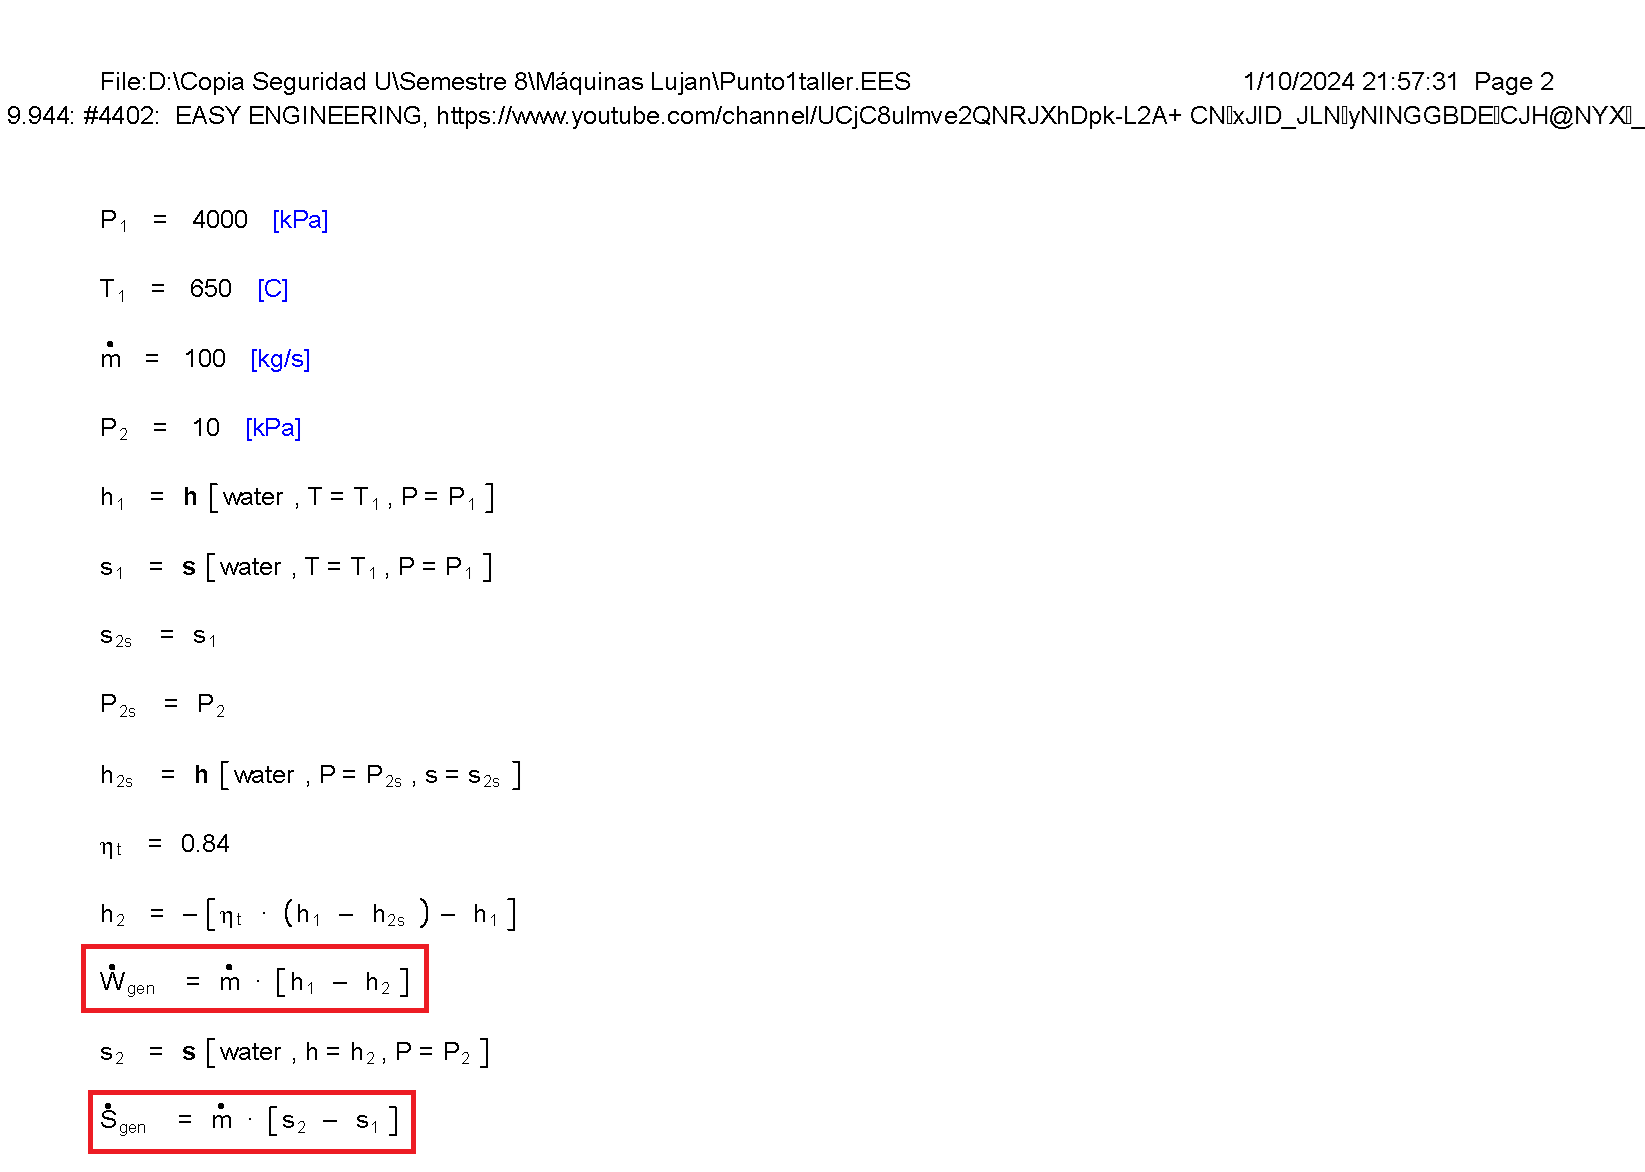
\includegraphics[width=1\textwidth]{equations.png} % Ajusta el ancho según necesites
            \caption{Datos y Ecuaciones en EES}
            \label{fig:mi_imagen}
        \end{figure}
        \newpage
        Para el estado 1 y 2:
        \begin{figure}[h!] % 'h' indica que LaTeX debe intentar colocar la figura aquí
            \centering
            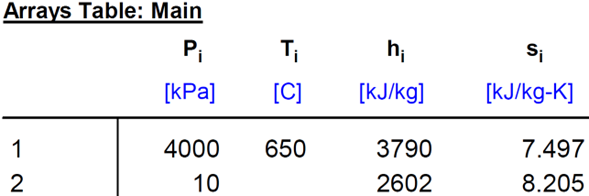
\includegraphics[width=1\textwidth]{arrays1.png} % Ajusta el ancho según necesites
            \caption{Estado 1 y Estado 2 en EES}
            \label{fig:mi_imagen}
        \end{figure}

        La solucion arrojada por EES, luego de despejar:
        \begin{figure}[h!] % 'h' indica que LaTeX debe intentar colocar la figura aquí
            \centering
            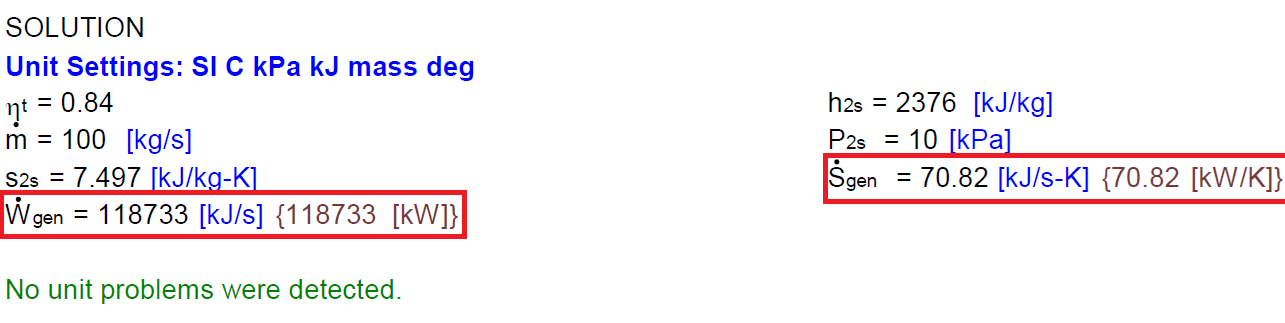
\includegraphics[width=1.1\textwidth]{solutions1.png} % Ajusta el ancho según necesites
            \caption{Solución en EES}
            \label{fig:mi_imagen}
        \end{figure}
\newpage
    \section*{1b}
    A continuación con herramientas de EES mostraremos ambos procesos sobre un diagrama h-s del agua, resaltamos las curvas isobáricas de 4 MPa y 10 kPa. Utilizando las herramientas <<Property Plot>> y <<Overlay Plot>> tenemos:
    \begin{figure}[h!] % 'h' indica que LaTeX debe intentar colocar la figura aquí
        \centering
        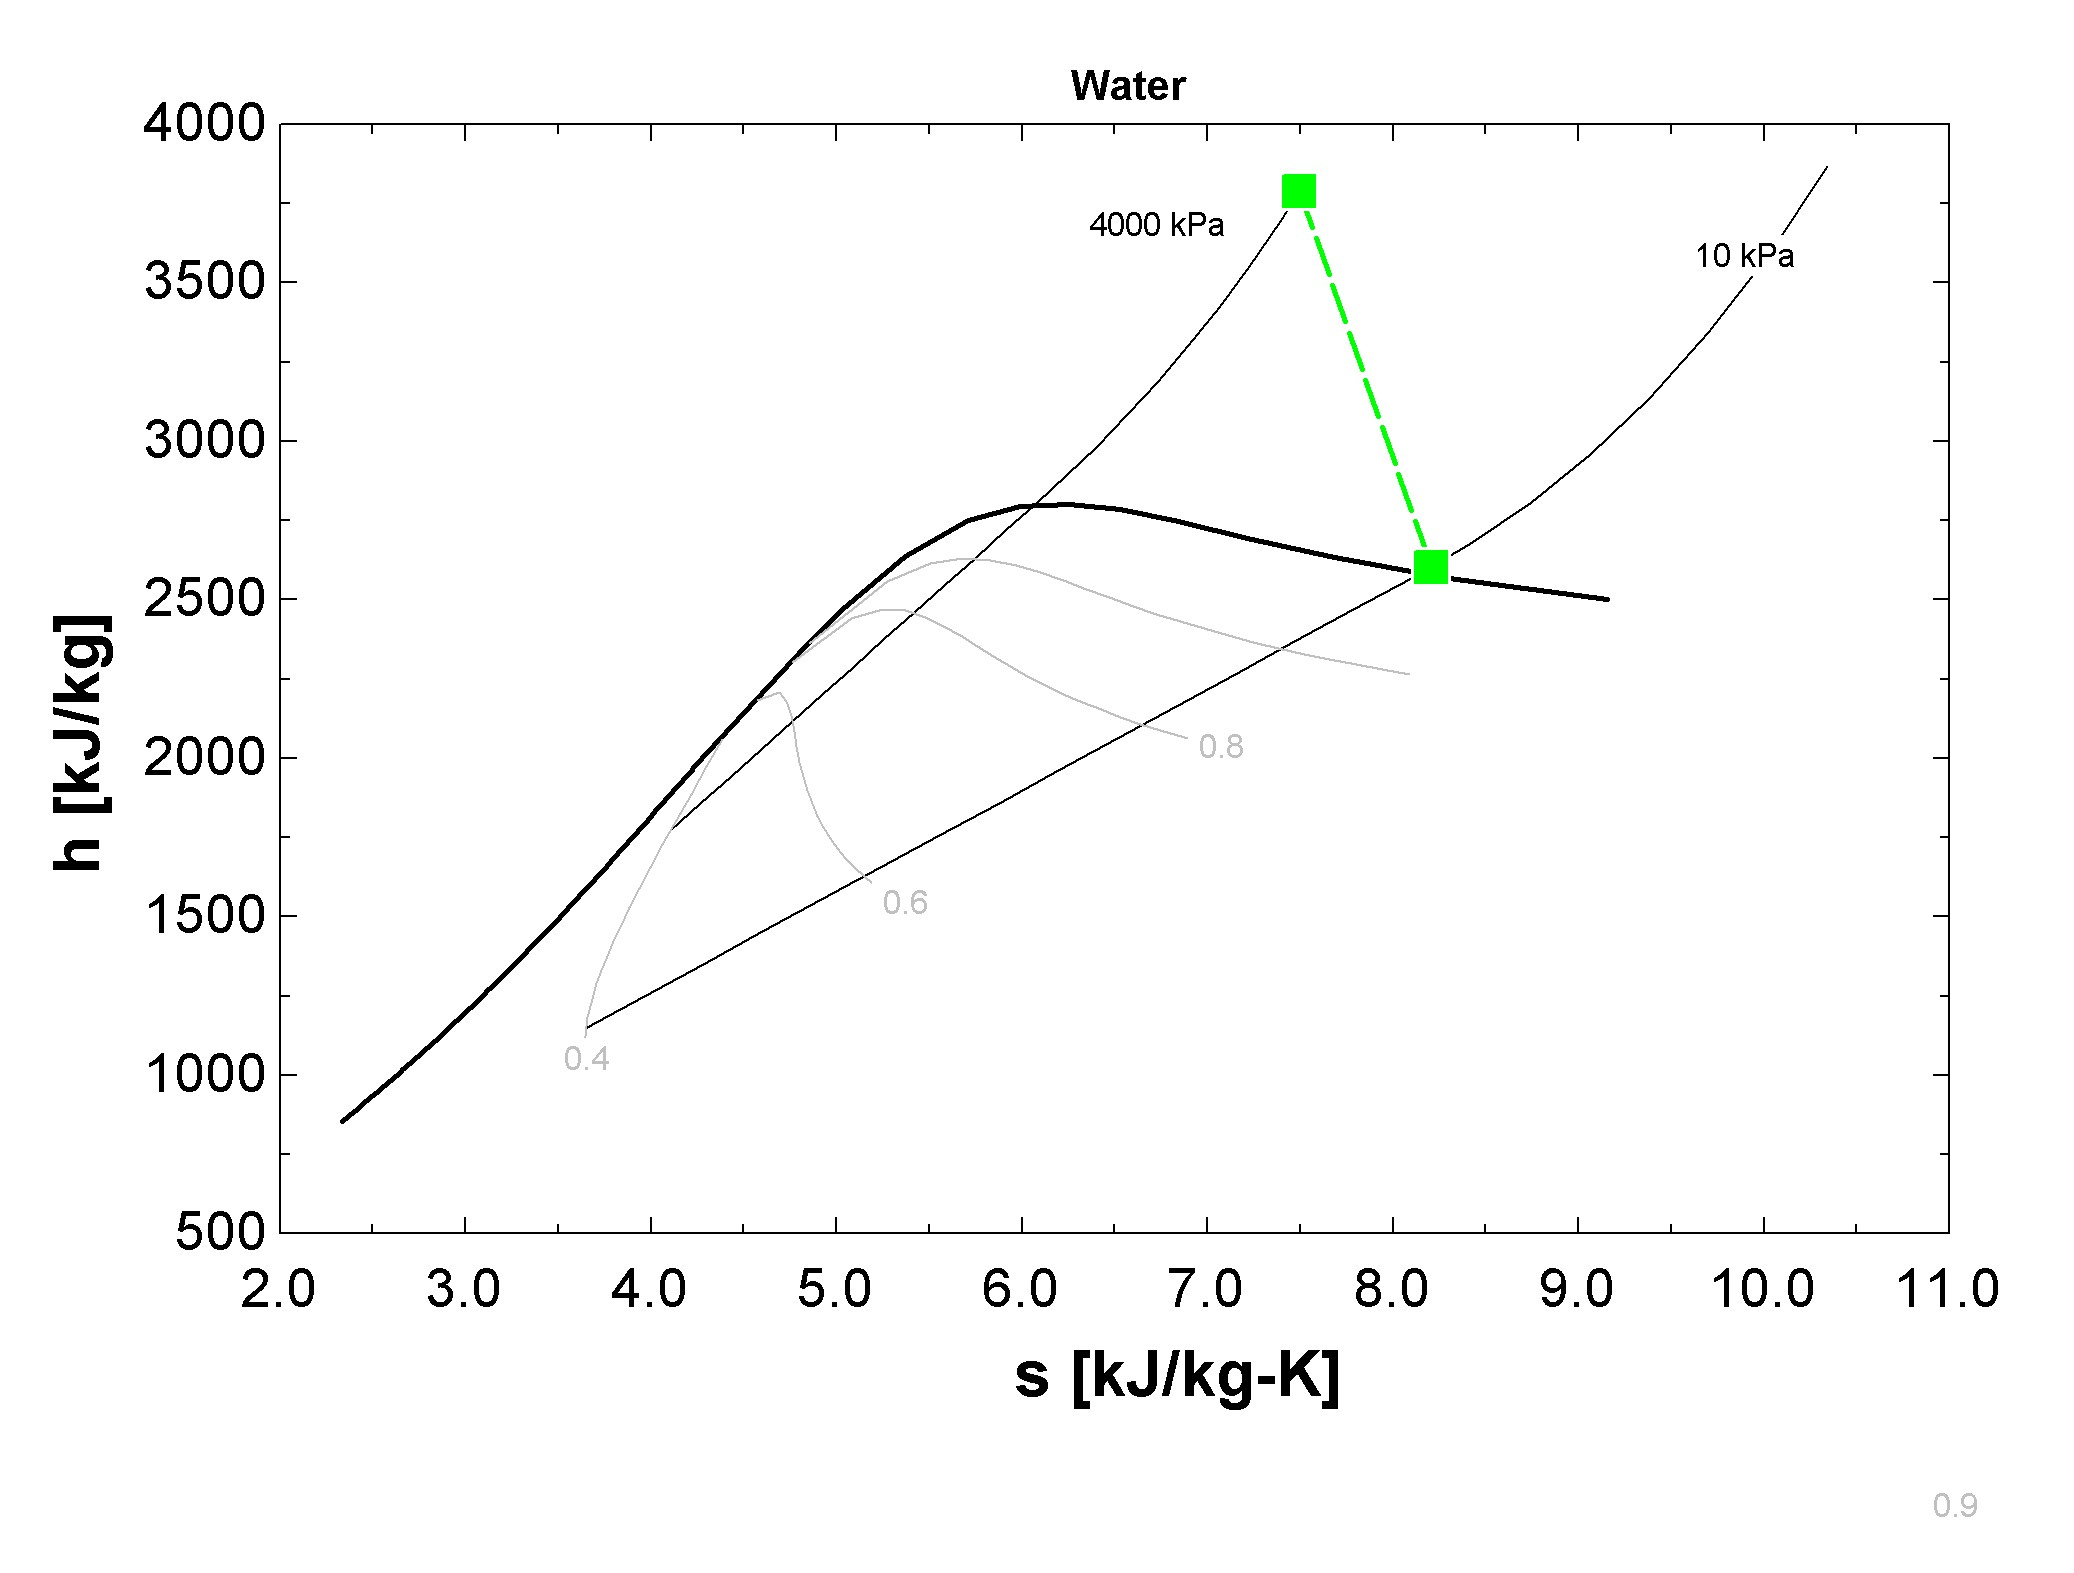
\includegraphics[width=1\textwidth]{hs.jpg} % Ajusta el ancho según necesites
        \caption{Gráfica h vs s}
        \label{fig:mi_imagen}
    \end{figure}
\newpage
\section{a,b}
Con el razonamiento y datos similares a los del primer punto y el concepto de relación de presiones en una turbina, lógica de programación (ciclos), el manual y el software de EES (Ciclo REPEAT). \singlespacing Procedemos a resolver el problema iterativo.
\begin{figure}[h!] % 'h' indica que LaTeX debe intentar colocar la figura aquí
    \centering
    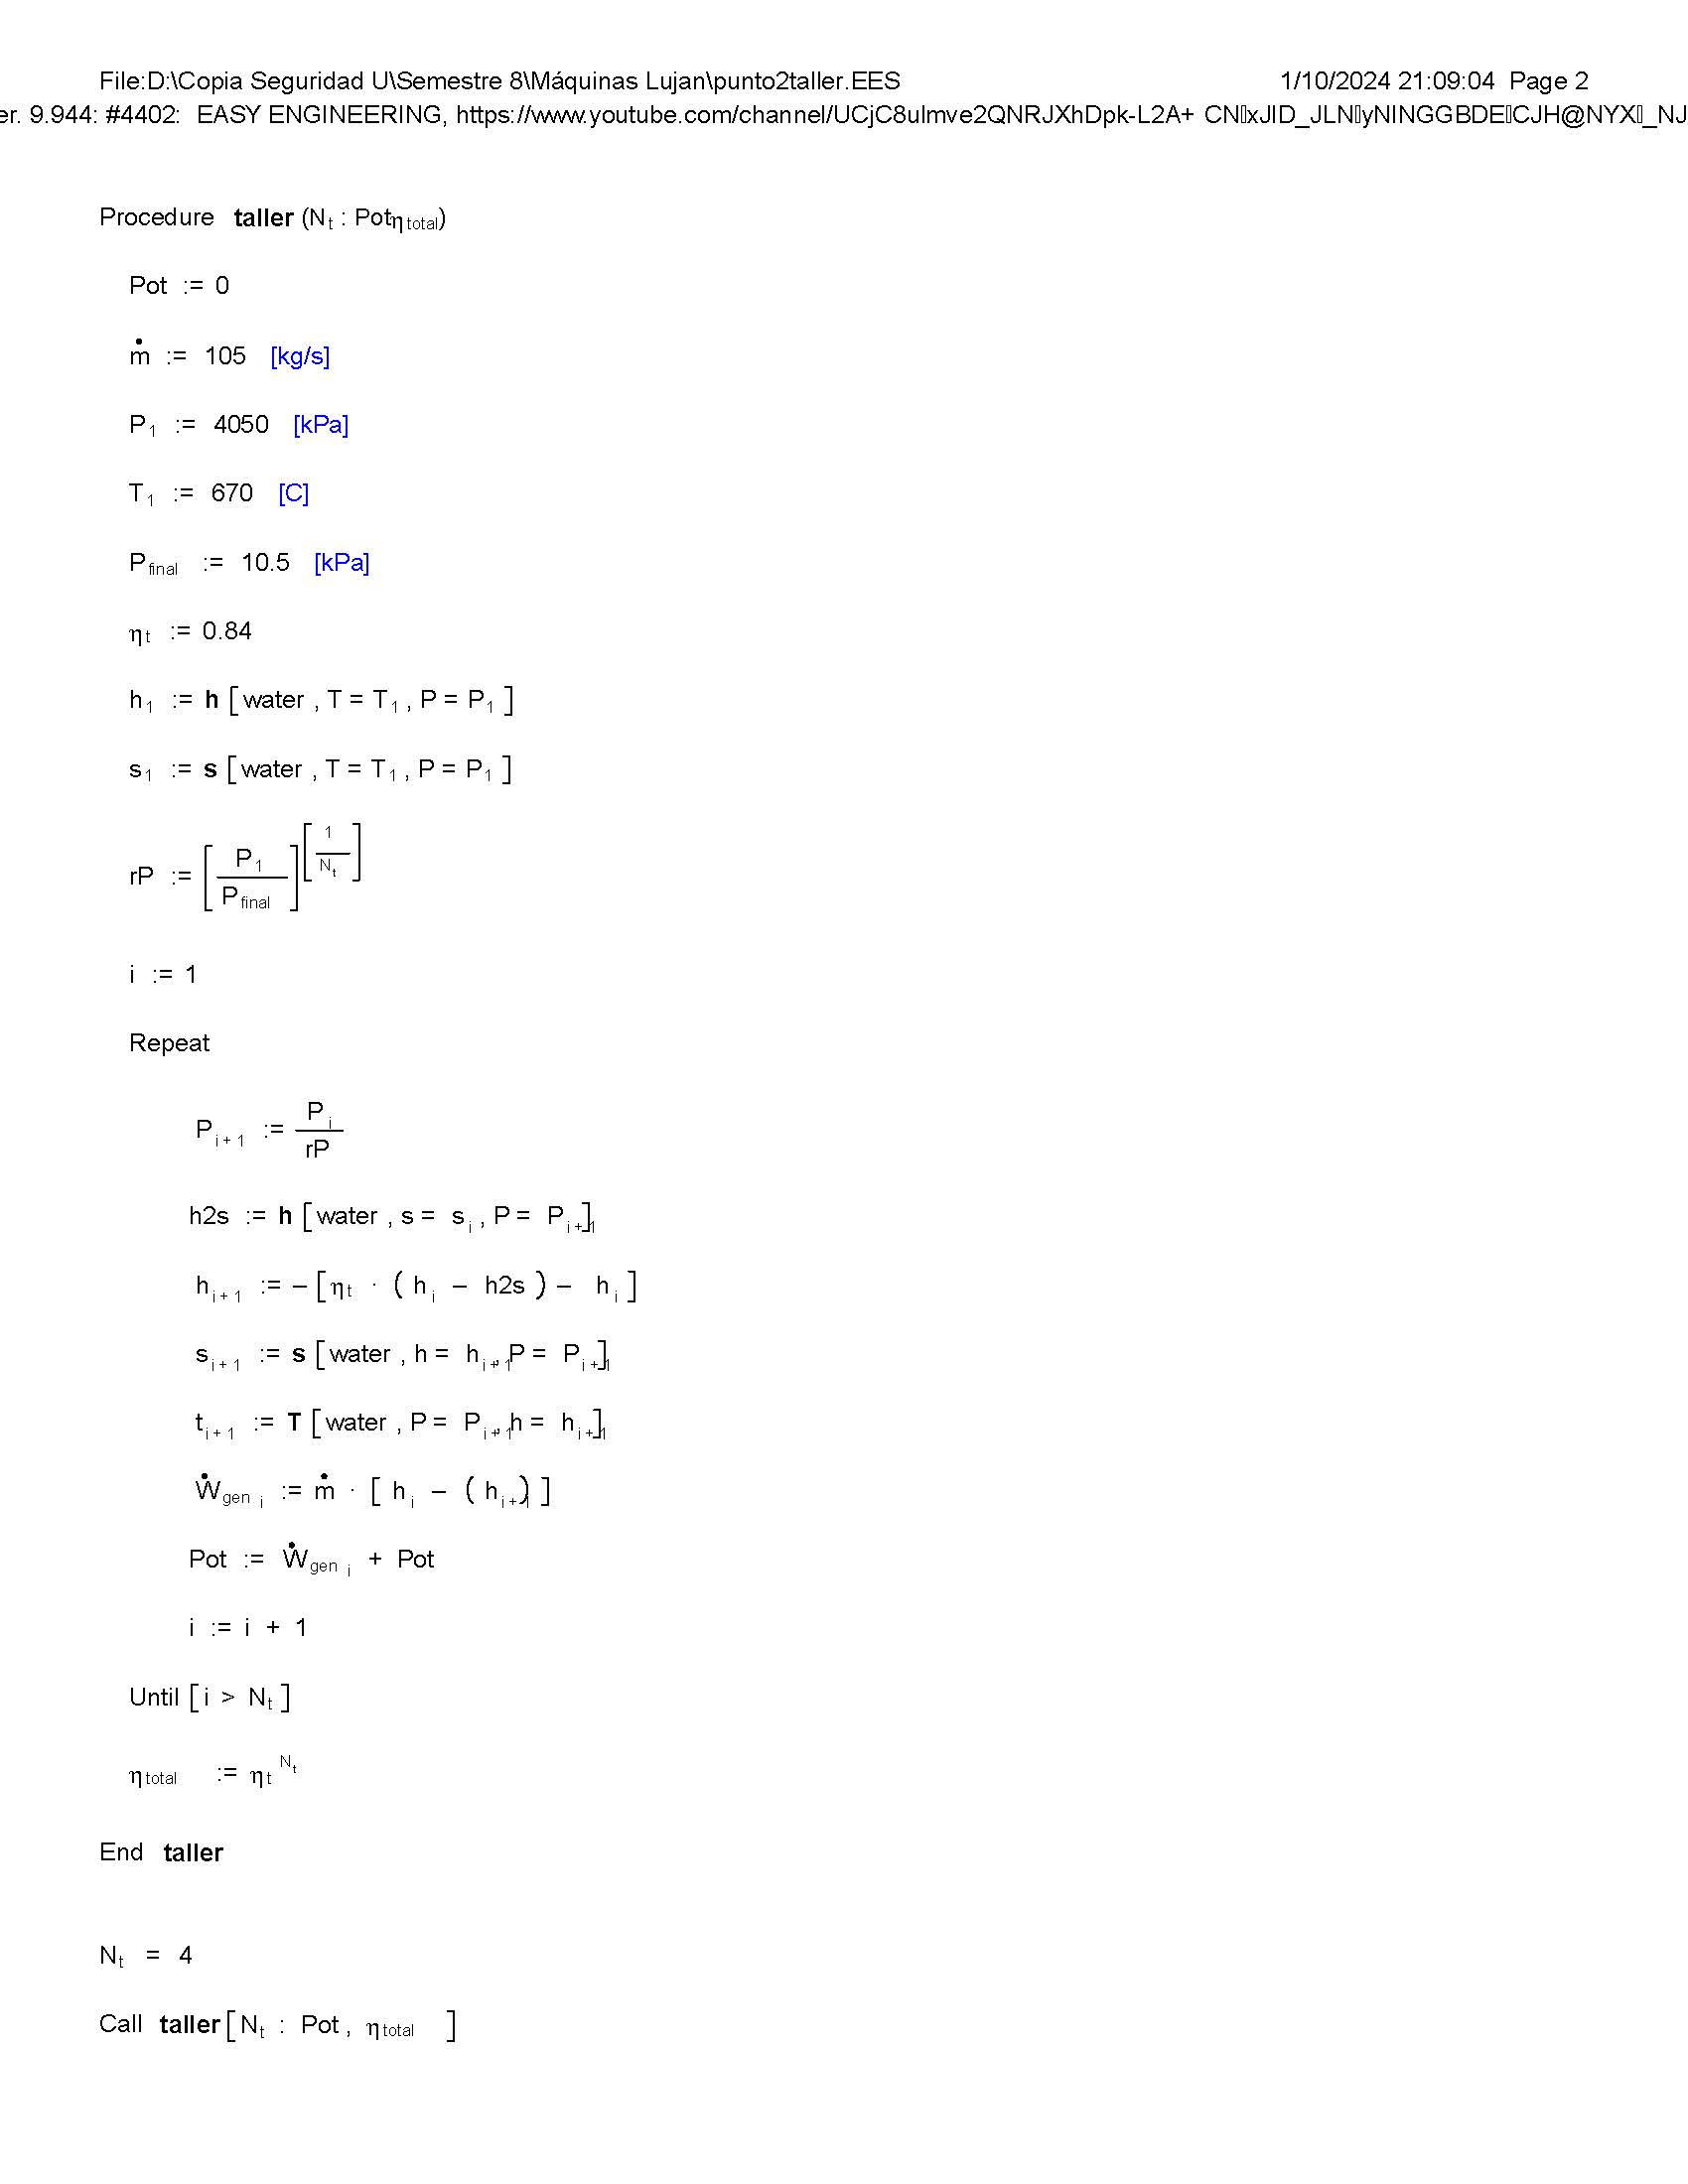
\includegraphics[width=0.8\textwidth]{ecuations222.jpg} % Ajusta el ancho según necesites
    \caption{Datos y Ecuaciones 2 en EES}
    \label{fig:mi_imagen}
\end{figure}
\newpage
La solución arrojada para la eficiencia Isentrópica total y potencia total del sistema, por EES, luego de despejar para N = 4 Turbinas:
\begin{figure}[h!] % 'h' indica que LaTeX debe intentar colocar la figura aquí
    \centering
    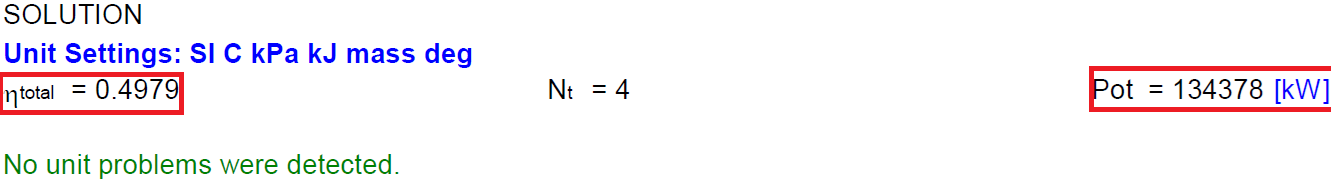
\includegraphics[width=1.1\textwidth]{solutions2.png} % Ajusta el ancho según necesites
    \caption{Solución 2 en EES}
    \label{fig:mi_imagen}
\end{figure}
\section*{2c.}
A continuación con herramientas de EES mostraremos los procesos sobre un diagrama h-s del agua, resaltamos las curvas isobáricas entre 4 MPa y 10 kPa. Utilizando las herramientas <<Property Plot>> y <<Overlay Plot>> tenemos:
\begin{figure}[h!] % 'h' indica que LaTeX debe intentar colocar la figura aquí
    \centering
    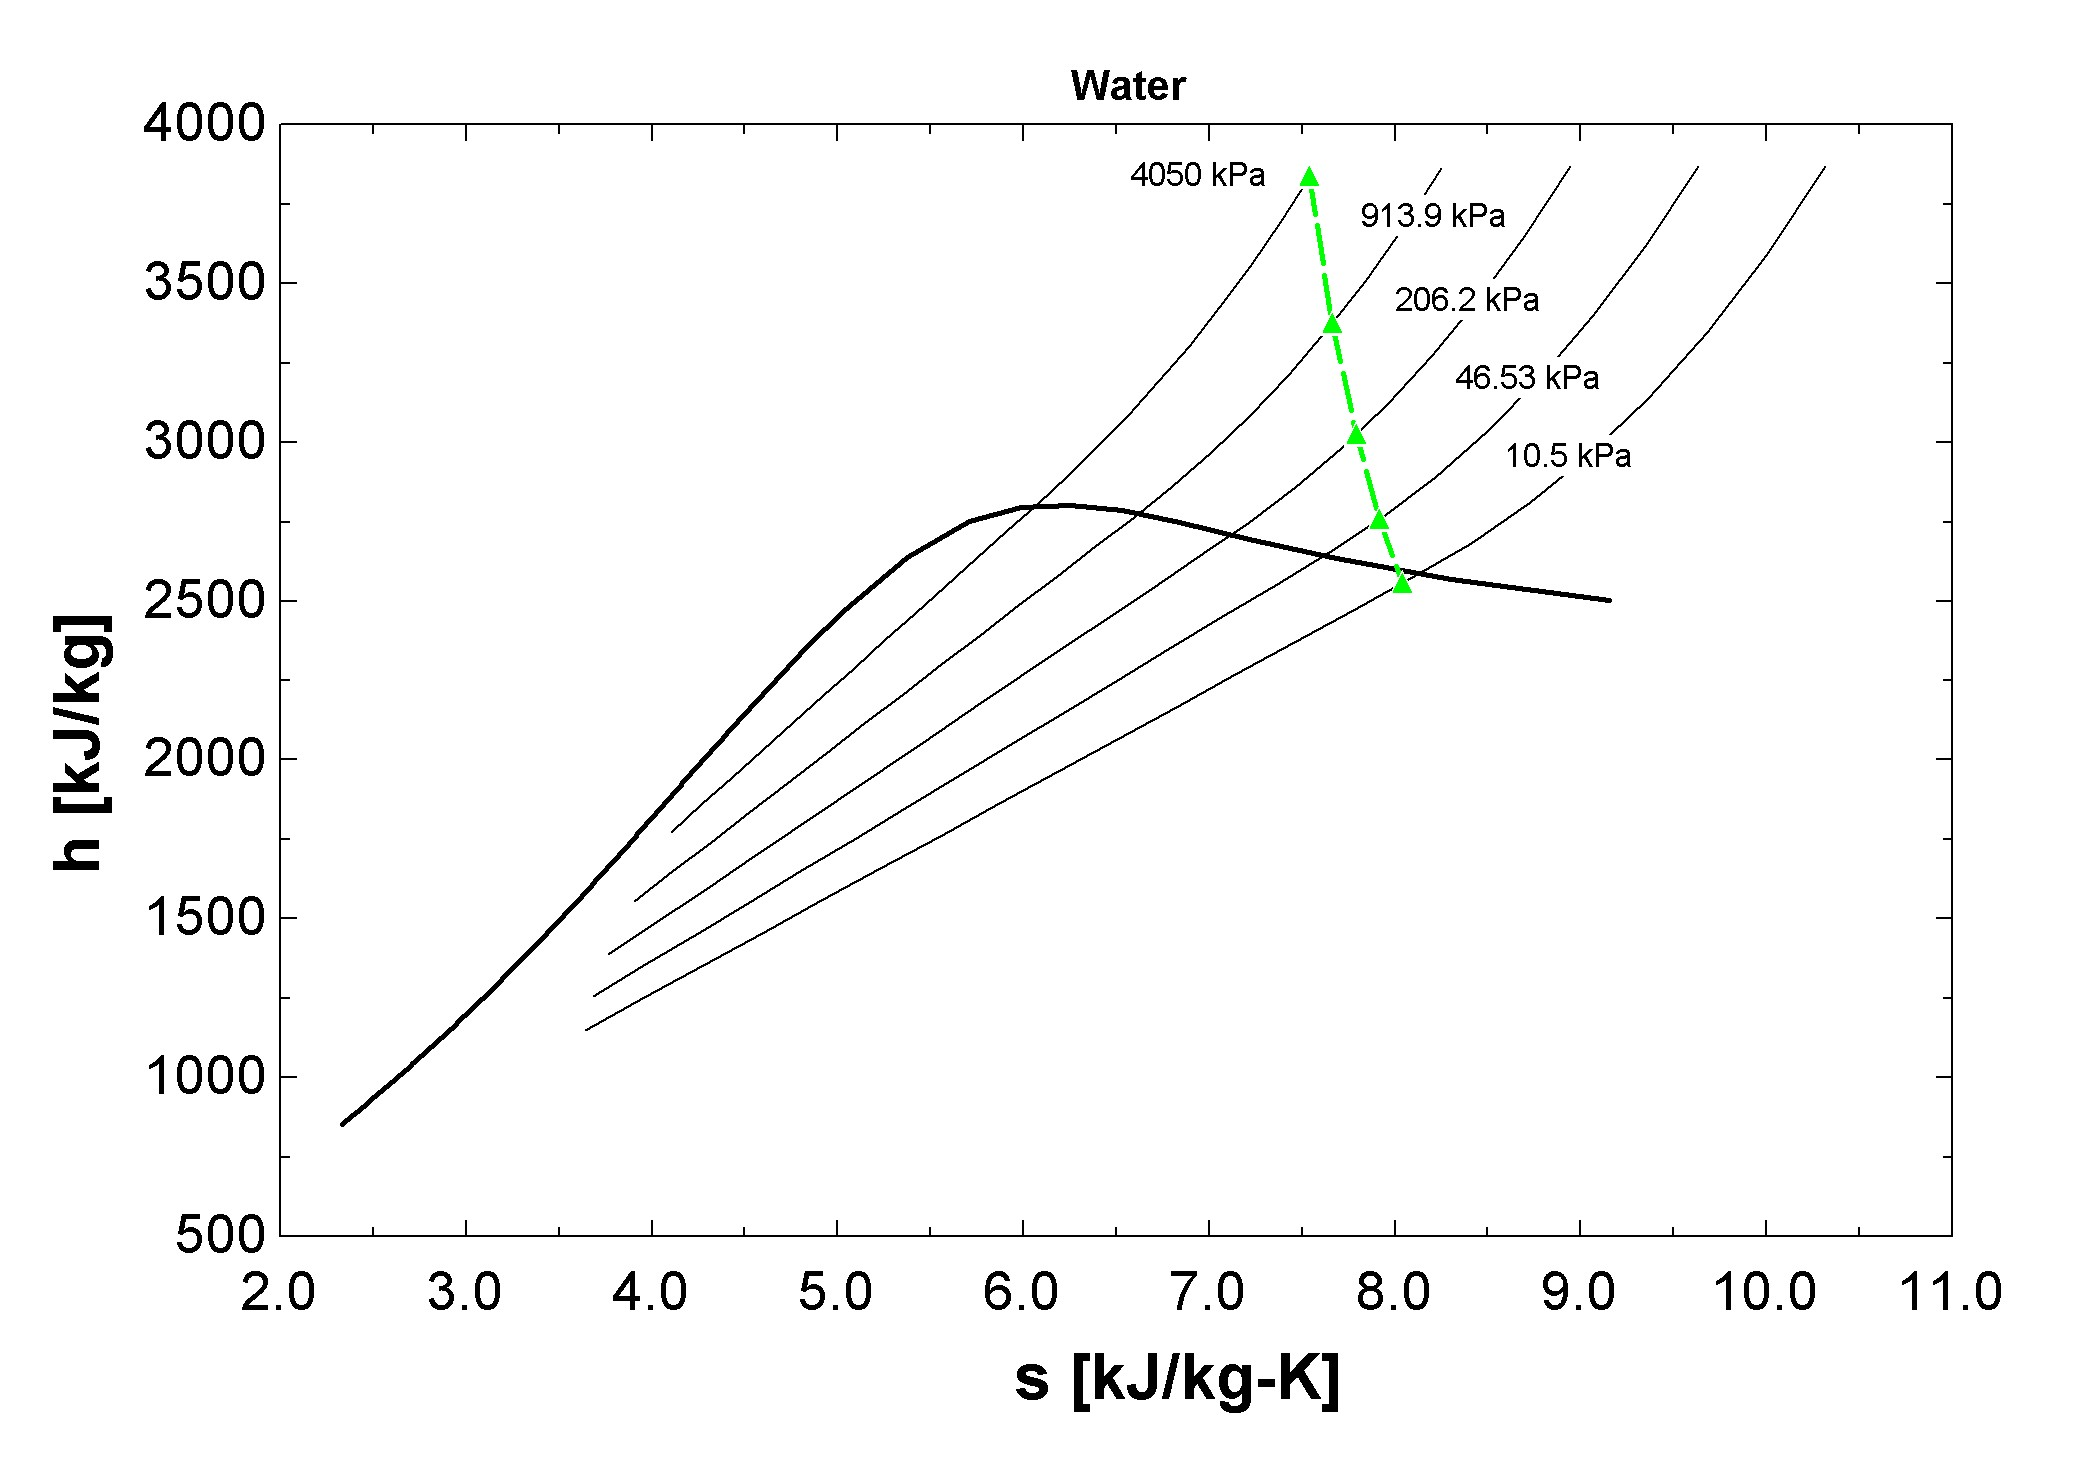
\includegraphics[width=1\textwidth]{h-s_4___TURBINAS.jpg} % Ajusta el ancho según necesites
    \caption{Gráfica para N=4 en EES}
    \label{fig:mi_imagen}
\end{figure}

\section*{2d.}
A continuación con herramientas de EES mostraremos un gráfico de la eficiencia isentrópica global en función del número de procesos de expansión (usando escala logarítmica en x y N de 1 a 100). Utilizando las herramientas <<X-Y Plot>> y <<Parametric Table>> tenemos:
\begin{figure}[h!] % 'h' indica que LaTeX debe intentar colocar la figura aquí
    \centering
    \includegraphics[width=1\textwidth]{Eficiencia_vs_Número_de_Turbinas2.jpg} % Ajusta el ancho según necesites
    \caption{Gráfica Eficiencia vs Número de Turbinas en EES}
    \label{fig:mi_imagen}
\end{figure}
\newpage
\bibliographystyle{apacite}
\nocite{*}
\bibliography{termodi}
\end{document}